\documentclass[1p]{elsarticle_modified}
%\bibliographystyle{elsarticle-num}

%\usepackage[colorlinks]{hyperref}
%\usepackage{abbrmath_seonhwa} %\Abb, \Ascr, \Acal ,\Abf, \Afrak
\usepackage{amsfonts}
\usepackage{amssymb}
\usepackage{amsmath}
\usepackage{amsthm}
\usepackage{scalefnt}
\usepackage{amsbsy}
\usepackage{kotex}
\usepackage{caption}
\usepackage{subfig}
\usepackage{color}
\usepackage{graphicx}
\usepackage{xcolor} %% white, black, red, green, blue, cyan, magenta, yellow
\usepackage{float}
\usepackage{setspace}
\usepackage{hyperref}

\usepackage{tikz}
\usetikzlibrary{arrows}

\usepackage{multirow}
\usepackage{array} % fixed length table
\usepackage{hhline}

%%%%%%%%%%%%%%%%%%%%%
\makeatletter
\renewcommand*\env@matrix[1][\arraystretch]{%
	\edef\arraystretch{#1}%
	\hskip -\arraycolsep
	\let\@ifnextchar\new@ifnextchar
	\array{*\c@MaxMatrixCols c}}
\makeatother %https://tex.stackexchange.com/questions/14071/how-can-i-increase-the-line-spacing-in-a-matrix
%%%%%%%%%%%%%%%

\usepackage[normalem]{ulem}

\newcommand{\msout}[1]{\ifmmode\text{\sout{\ensuremath{#1}}}\else\sout{#1}\fi}
%SOURCE: \msout is \stkout macro in https://tex.stackexchange.com/questions/20609/strikeout-in-math-mode

\newcommand{\cancel}[1]{
	\ifmmode
	{\color{red}\msout{#1}}
	\else
	{\color{red}\sout{#1}}
	\fi
}

\newcommand{\add}[1]{
	{\color{blue}\uwave{#1}}
}

\newcommand{\replace}[2]{
	\ifmmode
	{\color{red}\msout{#1}}{\color{blue}\uwave{#2}}
	\else
	{\color{red}\sout{#1}}{\color{blue}\uwave{#2}}
	\fi
}

\newcommand{\Sol}{\mathcal{S}} %segment
\newcommand{\D}{D} %diagram
\newcommand{\A}{\mathcal{A}} %arc


%%%%%%%%%%%%%%%%%%%%%%%%%%%%%5 test

\def\sl{\operatorname{\textup{SL}}(2,\Cbb)}
\def\psl{\operatorname{\textup{PSL}}(2,\Cbb)}
\def\quan{\mkern 1mu \triangleright \mkern 1mu}

\theoremstyle{definition}
\newtheorem{thm}{Theorem}[section]
\newtheorem{prop}[thm]{Proposition}
\newtheorem{lem}[thm]{Lemma}
\newtheorem{ques}[thm]{Question}
\newtheorem{cor}[thm]{Corollary}
\newtheorem{defn}[thm]{Definition}
\newtheorem{exam}[thm]{Example}
\newtheorem{rmk}[thm]{Remark}
\newtheorem{alg}[thm]{Algorithm}

\newcommand{\I}{\sqrt{-1}}
\begin{document}

%\begin{frontmatter}
%
%\title{Boundary parabolic representations of knots up to 8 crossings}
%
%%% Group authors per affiliation:
%\author{Yunhi Cho} 
%\address{Department of Mathematics, University of Seoul, Seoul, Korea}
%\ead{yhcho@uos.ac.kr}
%
%
%\author{Seonhwa Kim} %\fnref{s_kim}}
%\address{Center for Geometry and Physics, Institute for Basic Science, Pohang, 37673, Korea}
%\ead{ryeona17@ibs.re.kr}
%
%\author{Hyuk Kim}
%\address{Department of Mathematical Sciences, Seoul National University, Seoul 08826, Korea}
%\ead{hyukkim@snu.ac.kr}
%
%\author{Seokbeom Yoon}
%\address{Department of Mathematical Sciences, Seoul National University, Seoul, 08826,  Korea}
%\ead{sbyoon15@snu.ac.kr}
%
%\begin{abstract}
%We find all boundary parabolic representation of knots up to 8 crossings.
%
%\end{abstract}
%\begin{keyword}
%    \MSC[2010] 57M25 
%\end{keyword}
%
%\end{frontmatter}

%\linenumbers
%\tableofcontents
%
\newcommand\colored[1]{\textcolor{white}{\rule[-0.35ex]{0.8em}{1.4ex}}\kern-0.8em\color{red} #1}%
%\newcommand\colored[1]{\textcolor{white}{ #1}\kern-2.17ex	\textcolor{white}{ #1}\kern-1.81ex	\textcolor{white}{ #1}\kern-2.15ex\color{red}#1	}

{\Large $\underline{12n_{0136}~(K12n_{0136})}$}

\setlength{\tabcolsep}{10pt}
\renewcommand{\arraystretch}{1.6}
\vspace{1cm}\begin{tabular}{m{100pt}>{\centering\arraybackslash}m{274pt}}
\multirow{5}{120pt}{
	\centering
	\includegraphics[width=112pt]{../../../GIT/diagram.site/Diagrams/png/2225_12n_0136.png}\\
\ \ \ A knot diagram\footnotemark}&
\allowdisplaybreaks
\textbf{Linearized knot diagam} \\
\cline{2-2}
 &
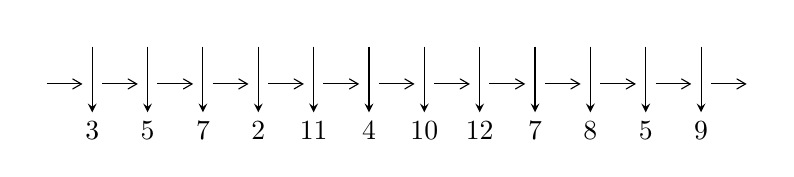
\begin{tikzpicture}[x=20pt, y=17pt]
	% nodes
	\node (C0) at (0, 0) {};
	\node (C1) at (1, 0) {};
	\node (C1U) at (1, +1) {};
	\node (C1D) at (1, -1) {3};

	\node (C2) at (2, 0) {};
	\node (C2U) at (2, +1) {};
	\node (C2D) at (2, -1) {5};

	\node (C3) at (3, 0) {};
	\node (C3U) at (3, +1) {};
	\node (C3D) at (3, -1) {7};

	\node (C4) at (4, 0) {};
	\node (C4U) at (4, +1) {};
	\node (C4D) at (4, -1) {2};

	\node (C5) at (5, 0) {};
	\node (C5U) at (5, +1) {};
	\node (C5D) at (5, -1) {11};

	\node (C6) at (6, 0) {};
	\node (C6U) at (6, +1) {};
	\node (C6D) at (6, -1) {4};

	\node (C7) at (7, 0) {};
	\node (C7U) at (7, +1) {};
	\node (C7D) at (7, -1) {10};

	\node (C8) at (8, 0) {};
	\node (C8U) at (8, +1) {};
	\node (C8D) at (8, -1) {12};

	\node (C9) at (9, 0) {};
	\node (C9U) at (9, +1) {};
	\node (C9D) at (9, -1) {7};

	\node (C10) at (10, 0) {};
	\node (C10U) at (10, +1) {};
	\node (C10D) at (10, -1) {8};

	\node (C11) at (11, 0) {};
	\node (C11U) at (11, +1) {};
	\node (C11D) at (11, -1) {5};

	\node (C12) at (12, 0) {};
	\node (C12U) at (12, +1) {};
	\node (C12D) at (12, -1) {9};
	\node (C13) at (13, 0) {};

	% arrows
	\draw[->,>={angle 60}]
	(C0) edge (C1) (C1) edge (C2) (C2) edge (C3) (C3) edge (C4) (C4) edge (C5) (C5) edge (C6) (C6) edge (C7) (C7) edge (C8) (C8) edge (C9) (C9) edge (C10) (C10) edge (C11) (C11) edge (C12) (C12) edge (C13) ;	\draw[->,>=stealth]
	(C1U) edge (C1D) (C2U) edge (C2D) (C3U) edge (C3D) (C4U) edge (C4D) (C5U) edge (C5D) (C6U) edge (C6D) (C7U) edge (C7D) (C8U) edge (C8D) (C9U) edge (C9D) (C10U) edge (C10D) (C11U) edge (C11D) (C12U) edge (C12D) ;
	\end{tikzpicture} \\
\hhline{~~} \\& 
\textbf{Solving Sequence} \\ \cline{2-2} 
 &
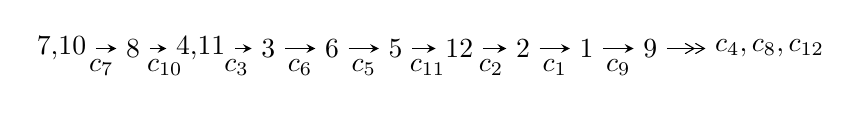
\begin{tikzpicture}[x=23pt, y=7pt]
	% node
	\node (A0) at (-1/8, 0) {7,10};
	\node (A1) at (1, 0) {8};
	\node (A2) at (33/16, 0) {4,11};
	\node (A3) at (25/8, 0) {3};
	\node (A4) at (33/8, 0) {6};
	\node (A5) at (41/8, 0) {5};
	\node (A6) at (49/8, 0) {12};
	\node (A7) at (57/8, 0) {2};
	\node (A8) at (65/8, 0) {1};
	\node (A9) at (73/8, 0) {9};
	\node (C1) at (1/2, -1) {$c_{7}$};
	\node (C2) at (3/2, -1) {$c_{10}$};
	\node (C3) at (21/8, -1) {$c_{3}$};
	\node (C4) at (29/8, -1) {$c_{6}$};
	\node (C5) at (37/8, -1) {$c_{5}$};
	\node (C6) at (45/8, -1) {$c_{11}$};
	\node (C7) at (53/8, -1) {$c_{2}$};
	\node (C8) at (61/8, -1) {$c_{1}$};
	\node (C9) at (69/8, -1) {$c_{9}$};
	\node (A10) at (11, 0) {$c_{4},c_{8},c_{12}$};

	% edge
	\draw[->,>=stealth]	
	(A0) edge (A1) (A1) edge (A2) (A2) edge (A3) (A3) edge (A4) (A4) edge (A5) (A5) edge (A6) (A6) edge (A7) (A7) edge (A8) (A8) edge (A9) ;
	\draw[->>,>={angle 60}]	
	(A9) edge (A10);
\end{tikzpicture} \\ 

\end{tabular} \\

\footnotetext{
The image of knot diagram is generated by the software ``\textbf{Draw programme}" developed by Andrew Bartholomew(\url{http://www.layer8.co.uk/maths/draw/index.htm\#Running-draw}), where we modified some parts for our purpose(\url{https://github.com/CATsTAILs/LinksPainter}).
}\phantom \\ \newline 
\centering \textbf{Ideals for irreducible components\footnotemark of $X_{\text{par}}$} 
 
\begin{align*}
I^u_{1}&=\langle 
-8.90997\times10^{57} u^{44}-6.51627\times10^{58} u^{43}+\cdots+1.48622\times10^{59} b+7.97191\times10^{58},\\
\phantom{I^u_{1}}&\phantom{= \langle  }1.29931\times10^{59} u^{44}+1.18228\times10^{60} u^{43}+\cdots+5.94490\times10^{59} a-4.97521\times10^{60},\;u^{45}+7 u^{44}+\cdots+12 u-1\rangle \\
I^u_{2}&=\langle 
b,\;3 u^7+5 u^6-7 u^5-11 u^4+5 u^3+3 u^2+a+7,\;u^8+u^7-3 u^6-2 u^5+3 u^4+2 u-1\rangle \\
I^u_{3}&=\langle 
5 a^2 u-3 a^2+12 a u+b-7 a+3 u-1,\;a^3- a^2 u+a^2+3 a u+6 a+3 u+5,\;u^2+u-1\rangle \\
I^u_{4}&=\langle 
b+a-2,\;a^2-3 a+1,\;u-1\rangle \\
\\
\end{align*}
\raggedright * 4 irreducible components of $\dim_{\mathbb{C}}=0$, with total 61 representations.\\
\footnotetext{All coefficients of polynomials are rational numbers. But the coefficients are sometimes approximated in decimal forms when there is not enough margin.}
\newpage
\renewcommand{\arraystretch}{1}
\centering \section*{I. $I^u_{1}= \langle -8.91\times10^{57} u^{44}-6.52\times10^{58} u^{43}+\cdots+1.49\times10^{59} b+7.97\times10^{58},\;1.30\times10^{59} u^{44}+1.18\times10^{60} u^{43}+\cdots+5.94\times10^{59} a-4.98\times10^{60},\;u^{45}+7 u^{44}+\cdots+12 u-1 \rangle$}
\flushleft \textbf{(i) Arc colorings}\\
\begin{tabular}{m{7pt} m{180pt} m{7pt} m{180pt} }
\flushright $a_{7}=$&$\begin{pmatrix}1\\0\end{pmatrix}$ \\
\flushright $a_{10}=$&$\begin{pmatrix}0\\u\end{pmatrix}$ \\
\flushright $a_{8}=$&$\begin{pmatrix}1\\u^2\end{pmatrix}$ \\
\flushright $a_{4}=$&$\begin{pmatrix}-0.218558 u^{44}-1.98872 u^{43}+\cdots-84.8505 u+8.36887\\0.0599504 u^{44}+0.438445 u^{43}+\cdots-0.981685 u-0.536386\end{pmatrix}$ \\
\flushright $a_{11}=$&$\begin{pmatrix}- u\\- u^3+u\end{pmatrix}$ \\
\flushright $a_{3}=$&$\begin{pmatrix}-0.158608 u^{44}-1.55028 u^{43}+\cdots-85.8322 u+7.83248\\0.0599504 u^{44}+0.438445 u^{43}+\cdots-0.981685 u-0.536386\end{pmatrix}$ \\
\flushright $a_{6}=$&$\begin{pmatrix}0.441060 u^{44}+3.11339 u^{43}+\cdots-65.1681 u+7.22415\\0.0840649 u^{44}+0.554982 u^{43}+\cdots-0.887359 u-0.303624\end{pmatrix}$ \\
\flushright $a_{5}=$&$\begin{pmatrix}0.519991 u^{44}+3.59140 u^{43}+\cdots-64.5950 u+7.21939\\0.0844612 u^{44}+0.574806 u^{43}+\cdots-0.487423 u-0.373377\end{pmatrix}$ \\
\flushright $a_{12}=$&$\begin{pmatrix}-0.131038 u^{44}-0.902044 u^{43}+\cdots+25.2448 u-3.79525\\-0.0152230 u^{44}-0.0901999 u^{43}+\cdots+2.22280 u+0.131038\end{pmatrix}$ \\
\flushright $a_{2}=$&$\begin{pmatrix}-0.365995 u^{44}-2.97364 u^{43}+\cdots-44.5369 u+4.24425\\0.0844612 u^{44}+0.574806 u^{43}+\cdots-0.487423 u-0.373377\end{pmatrix}$ \\
\flushright $a_{1}=$&$\begin{pmatrix}0.0782668 u^{44}+0.573436 u^{43}+\cdots-25.1426 u+3.79639\\-0.0375483 u^{44}-0.238408 u^{43}+\cdots-2.12064 u-0.129900\end{pmatrix}$ \\
\flushright $a_{9}=$&$\begin{pmatrix}u\\u\end{pmatrix}$\\&\end{tabular}
\flushleft \textbf{(ii) Obstruction class $= -1$}\\~\\
\flushleft \textbf{(iii) Cusp Shapes $= 10.5915 u^{44}+78.5347 u^{43}+\cdots-186.556 u+9.63178$}\\~\\
\newpage\renewcommand{\arraystretch}{1}
\flushleft \textbf{(iv) u-Polynomials at the component}\newline \\
\begin{tabular}{m{50pt}|m{274pt}}
Crossings & \hspace{64pt}u-Polynomials at each crossing \\
\hline $$\begin{aligned}c_{1}\end{aligned}$$&$\begin{aligned}
&u^{45}+10 u^{44}+\cdots+930 u+1
\end{aligned}$\\
\hline $$\begin{aligned}c_{2},c_{4}\end{aligned}$$&$\begin{aligned}
&u^{45}-12 u^{44}+\cdots-26 u-1
\end{aligned}$\\
\hline $$\begin{aligned}c_{3},c_{6}\end{aligned}$$&$\begin{aligned}
&u^{45}-4 u^{44}+\cdots-640 u-256
\end{aligned}$\\
\hline $$\begin{aligned}c_{5},c_{11}\end{aligned}$$&$\begin{aligned}
&u^{45}-3 u^{44}+\cdots+32 u-64
\end{aligned}$\\
\hline $$\begin{aligned}c_{7},c_{9},c_{10}\end{aligned}$$&$\begin{aligned}
&u^{45}-7 u^{44}+\cdots+12 u+1
\end{aligned}$\\
\hline $$\begin{aligned}c_{8},c_{12}\end{aligned}$$&$\begin{aligned}
&u^{45}+5 u^{44}+\cdots-4 u-4
\end{aligned}$\\
\hline
\end{tabular}\\~\\
\newpage\renewcommand{\arraystretch}{1}
\flushleft \textbf{(v) Riley Polynomials at the component}\newline \\
\begin{tabular}{m{50pt}|m{274pt}}
Crossings & \hspace{64pt}Riley Polynomials at each crossing \\
\hline $$\begin{aligned}c_{1}\end{aligned}$$&$\begin{aligned}
&y^{45}+62 y^{44}+\cdots+852778 y-1
\end{aligned}$\\
\hline $$\begin{aligned}c_{2},c_{4}\end{aligned}$$&$\begin{aligned}
&y^{45}-10 y^{44}+\cdots+930 y-1
\end{aligned}$\\
\hline $$\begin{aligned}c_{3},c_{6}\end{aligned}$$&$\begin{aligned}
&y^{45}+54 y^{44}+\cdots+4571136 y-65536
\end{aligned}$\\
\hline $$\begin{aligned}c_{5},c_{11}\end{aligned}$$&$\begin{aligned}
&y^{45}+33 y^{44}+\cdots+234496 y-4096
\end{aligned}$\\
\hline $$\begin{aligned}c_{7},c_{9},c_{10}\end{aligned}$$&$\begin{aligned}
&y^{45}-31 y^{44}+\cdots-142 y-1
\end{aligned}$\\
\hline $$\begin{aligned}c_{8},c_{12}\end{aligned}$$&$\begin{aligned}
&y^{45}+3 y^{44}+\cdots+1256 y-16
\end{aligned}$\\
\hline
\end{tabular}\\~\\
\newpage\flushleft \textbf{(vi) Complex Volumes and Cusp Shapes}
$$\begin{array}{c|c|c}  
\text{Solutions to }I^u_{1}& \I (\text{vol} + \sqrt{-1}CS) & \text{Cusp shape}\\
 \hline 
\begin{aligned}
u &= \phantom{-}0.989081\phantom{ +0.000000I} \\
a &= \phantom{-}5.39659\phantom{ +0.000000I} \\
b &= -0.601818\phantom{ +0.000000I}\end{aligned}
 & -2.67208\phantom{ +0.000000I} & -212.850\phantom{ +0.000000I} \\ \hline\begin{aligned}
u &= \phantom{-}0.952866 + 0.134525 I \\
a &= -4.15928 - 0.51646 I \\
b &= -0.377187 + 0.281972 I\end{aligned}
 & -2.91440 - 0.52040 I & -28.2057 - 17.3785 I \\ \hline\begin{aligned}
u &= \phantom{-}0.952866 - 0.134525 I \\
a &= -4.15928 + 0.51646 I \\
b &= -0.377187 - 0.281972 I\end{aligned}
 & -2.91440 + 0.52040 I & -28.2057 + 17.3785 I \\ \hline\begin{aligned}
u &= -1.04539\phantom{ +0.000000I} \\
a &= \phantom{-}0.313771\phantom{ +0.000000I} \\
b &= \phantom{-}1.54859\phantom{ +0.000000I}\end{aligned}
 & -10.6185\phantom{ +0.000000I} & -59.2780\phantom{ +0.000000I} \\ \hline\begin{aligned}
u &= -0.367366 + 0.850305 I \\
a &= -0.393666 + 0.059604 I \\
b &= \phantom{-}1.16026 + 0.81675 I\end{aligned}
 & \phantom{-}4.19700 - 1.34910 I & -7.72837 + 1.14036 I \\ \hline\begin{aligned}
u &= -0.367366 - 0.850305 I \\
a &= -0.393666 - 0.059604 I \\
b &= \phantom{-}1.16026 - 0.81675 I\end{aligned}
 & \phantom{-}4.19700 + 1.34910 I & -7.72837 - 1.14036 I \\ \hline\begin{aligned}
u &= -0.626112 + 0.680342 I \\
a &= \phantom{-}1.12492 + 1.02026 I \\
b &= \phantom{-}0.00967 - 1.90333 I\end{aligned}
 & \phantom{-}5.86522 - 1.45260 I & -9.17004 + 0.17720 I \\ \hline\begin{aligned}
u &= -0.626112 - 0.680342 I \\
a &= \phantom{-}1.12492 - 1.02026 I \\
b &= \phantom{-}0.00967 + 1.90333 I\end{aligned}
 & \phantom{-}5.86522 + 1.45260 I & -9.17004 - 0.17720 I \\ \hline\begin{aligned}
u &= -0.952838 + 0.522259 I \\
a &= \phantom{-}0.132474 + 0.580825 I \\
b &= -0.51946 - 1.36700 I\end{aligned}
 & -0.90351 + 3.78658 I & -12.00000 - 4.56976 I \\ \hline\begin{aligned}
u &= -0.952838 - 0.522259 I \\
a &= \phantom{-}0.132474 - 0.580825 I \\
b &= -0.51946 + 1.36700 I\end{aligned}
 & -0.90351 - 3.78658 I & -12.00000 + 4.56976 I\\
 \hline 
 \end{array}$$\newpage$$\begin{array}{c|c|c}  
\text{Solutions to }I^u_{1}& \I (\text{vol} + \sqrt{-1}CS) & \text{Cusp shape}\\
 \hline 
\begin{aligned}
u &= \phantom{-}1.007870 + 0.493819 I \\
a &= \phantom{-}0.985859 - 0.555848 I \\
b &= \phantom{-}0.560995 + 0.542777 I\end{aligned}
 & -0.360727 - 0.771902 I & -12.00000 + 0. I\phantom{ +0.000000I} \\ \hline\begin{aligned}
u &= \phantom{-}1.007870 - 0.493819 I \\
a &= \phantom{-}0.985859 + 0.555848 I \\
b &= \phantom{-}0.560995 - 0.542777 I\end{aligned}
 & -0.360727 + 0.771902 I & -12.00000 + 0. I\phantom{ +0.000000I} \\ \hline\begin{aligned}
u &= -0.973372 + 0.572106 I \\
a &= -1.06022 - 0.96272 I \\
b &= -0.62624 + 1.82528 I\end{aligned}
 & \phantom{-}4.81861 + 6.30906 I & -12.00000 - 5.34980 I \\ \hline\begin{aligned}
u &= -0.973372 - 0.572106 I \\
a &= -1.06022 + 0.96272 I \\
b &= -0.62624 - 1.82528 I\end{aligned}
 & \phantom{-}4.81861 - 6.30906 I & -12.00000 + 5.34980 I \\ \hline\begin{aligned}
u &= -0.668847 + 0.501935 I \\
a &= -1.094700 - 0.761183 I \\
b &= -1.200670 + 0.692757 I\end{aligned}
 & -0.018874 + 0.450301 I & -9.70033 - 2.11767 I \\ \hline\begin{aligned}
u &= -0.668847 - 0.501935 I \\
a &= -1.094700 + 0.761183 I \\
b &= -1.200670 - 0.692757 I\end{aligned}
 & -0.018874 - 0.450301 I & -9.70033 + 2.11767 I \\ \hline\begin{aligned}
u &= \phantom{-}0.781094 + 0.070241 I \\
a &= -0.13334 + 3.27365 I \\
b &= -0.197314 - 1.345870 I\end{aligned}
 & \phantom{-}1.89233 - 2.90725 I & -43.5907 + 10.5695 I \\ \hline\begin{aligned}
u &= \phantom{-}0.781094 - 0.070241 I \\
a &= -0.13334 - 3.27365 I \\
b &= -0.197314 + 1.345870 I\end{aligned}
 & \phantom{-}1.89233 + 2.90725 I & -43.5907 - 10.5695 I \\ \hline\begin{aligned}
u &= \phantom{-}0.068357 + 1.251150 I \\
a &= -0.00386 - 1.50825 I \\
b &= \phantom{-}0.59331 + 1.89133 I\end{aligned}
 & \phantom{-}12.3107 - 8.8025 I & \phantom{-0.000000 } 0 \\ \hline\begin{aligned}
u &= \phantom{-}0.068357 - 1.251150 I \\
a &= -0.00386 + 1.50825 I \\
b &= \phantom{-}0.59331 - 1.89133 I\end{aligned}
 & \phantom{-}12.3107 + 8.8025 I & \phantom{-0.000000 } 0\\
 \hline 
 \end{array}$$\newpage$$\begin{array}{c|c|c}  
\text{Solutions to }I^u_{1}& \I (\text{vol} + \sqrt{-1}CS) & \text{Cusp shape}\\
 \hline 
\begin{aligned}
u &= -0.139719 + 1.259590 I \\
a &= \phantom{-}0.22206 + 1.51967 I \\
b &= \phantom{-}0.04895 - 2.08421 I\end{aligned}
 & \phantom{-}13.18790 - 0.68473 I & \phantom{-0.000000 } 0 \\ \hline\begin{aligned}
u &= -0.139719 - 1.259590 I \\
a &= \phantom{-}0.22206 - 1.51967 I \\
b &= \phantom{-}0.04895 + 2.08421 I\end{aligned}
 & \phantom{-}13.18790 + 0.68473 I & \phantom{-0.000000 } 0 \\ \hline\begin{aligned}
u &= \phantom{-}0.306575 + 0.653371 I \\
a &= \phantom{-}0.163852 + 0.671962 I \\
b &= -0.009810 - 0.890868 I\end{aligned}
 & \phantom{-}1.38833 - 3.58772 I & -7.79003 + 7.62926 I \\ \hline\begin{aligned}
u &= \phantom{-}0.306575 - 0.653371 I \\
a &= \phantom{-}0.163852 - 0.671962 I \\
b &= -0.009810 + 0.890868 I\end{aligned}
 & \phantom{-}1.38833 + 3.58772 I & -7.79003 - 7.62926 I \\ \hline\begin{aligned}
u &= -1.141470 + 0.620472 I \\
a &= \phantom{-}0.459135 + 0.678243 I \\
b &= \phantom{-}1.58964 - 0.23048 I\end{aligned}
 & \phantom{-}1.89448 + 6.79376 I & \phantom{-0.000000 } 0 \\ \hline\begin{aligned}
u &= -1.141470 - 0.620472 I \\
a &= \phantom{-}0.459135 - 0.678243 I \\
b &= \phantom{-}1.58964 + 0.23048 I\end{aligned}
 & \phantom{-}1.89448 - 6.79376 I & \phantom{-0.000000 } 0 \\ \hline\begin{aligned}
u &= \phantom{-}1.300200 + 0.172788 I \\
a &= \phantom{-}0.174045 - 0.780639 I \\
b &= \phantom{-}0.189316 - 0.701955 I\end{aligned}
 & -1.23770 - 1.72442 I & \phantom{-0.000000 } 0 \\ \hline\begin{aligned}
u &= \phantom{-}1.300200 - 0.172788 I \\
a &= \phantom{-}0.174045 + 0.780639 I \\
b &= \phantom{-}0.189316 + 0.701955 I\end{aligned}
 & -1.23770 + 1.72442 I & \phantom{-0.000000 } 0 \\ \hline\begin{aligned}
u &= -1.353400 + 0.275389 I \\
a &= -0.297373 + 0.170909 I \\
b &= -0.179271 + 0.620523 I\end{aligned}
 & -3.67456 + 6.89597 I & \phantom{-0.000000 } 0 \\ \hline\begin{aligned}
u &= -1.353400 - 0.275389 I \\
a &= -0.297373 - 0.170909 I \\
b &= -0.179271 - 0.620523 I\end{aligned}
 & -3.67456 - 6.89597 I & \phantom{-0.000000 } 0\\
 \hline 
 \end{array}$$\newpage$$\begin{array}{c|c|c}  
\text{Solutions to }I^u_{1}& \I (\text{vol} + \sqrt{-1}CS) & \text{Cusp shape}\\
 \hline 
\begin{aligned}
u &= \phantom{-}0.532389\phantom{ +0.000000I} \\
a &= \phantom{-}10.6740\phantom{ +0.000000I} \\
b &= \phantom{-}0.157357\phantom{ +0.000000I}\end{aligned}
 & -2.53079\phantom{ +0.000000I} & -190.200\phantom{ +0.000000I} \\ \hline\begin{aligned}
u &= -1.52798 + 0.15122 I \\
a &= \phantom{-}0.328835 + 0.021672 I \\
b &= -0.203375 - 1.016320 I\end{aligned}
 & -6.72932 + 1.63796 I & \phantom{-0.000000 } 0 \\ \hline\begin{aligned}
u &= -1.52798 - 0.15122 I \\
a &= \phantom{-}0.328835 - 0.021672 I \\
b &= -0.203375 + 1.016320 I\end{aligned}
 & -6.72932 - 1.63796 I & \phantom{-0.000000 } 0 \\ \hline\begin{aligned}
u &= -1.36799 + 0.70186 I \\
a &= -0.945282 - 0.712027 I \\
b &= -0.35731 + 1.99808 I\end{aligned}
 & \phantom{-}9.42541 + 7.53688 I & \phantom{-0.000000 } 0 \\ \hline\begin{aligned}
u &= -1.36799 - 0.70186 I \\
a &= -0.945282 + 0.712027 I \\
b &= -0.35731 - 1.99808 I\end{aligned}
 & \phantom{-}9.42541 - 7.53688 I & \phantom{-0.000000 } 0 \\ \hline\begin{aligned}
u &= -1.45214 + 0.59473 I \\
a &= \phantom{-}1.17477 + 0.82015 I \\
b &= \phantom{-}0.78255 - 1.69623 I\end{aligned}
 & \phantom{-}7.5666 + 15.2974 I & \phantom{-0.000000 } 0 \\ \hline\begin{aligned}
u &= -1.45214 - 0.59473 I \\
a &= \phantom{-}1.17477 - 0.82015 I \\
b &= \phantom{-}0.78255 + 1.69623 I\end{aligned}
 & \phantom{-}7.5666 - 15.2974 I & \phantom{-0.000000 } 0 \\ \hline\begin{aligned}
u &= \phantom{-}0.409223\phantom{ +0.000000I} \\
a &= \phantom{-}1.48110\phantom{ +0.000000I} \\
b &= -0.181306\phantom{ +0.000000I}\end{aligned}
 & -0.821501\phantom{ +0.000000I} & -11.8740\phantom{ +0.000000I} \\ \hline\begin{aligned}
u &= \phantom{-}1.43589 + 0.72409 I \\
a &= -0.688447 + 0.406430 I \\
b &= \phantom{-}0.24206 - 1.91261 I\end{aligned}
 & \phantom{-}8.18611 + 1.85592 I & \phantom{-0.000000 } 0 \\ \hline\begin{aligned}
u &= \phantom{-}1.43589 - 0.72409 I \\
a &= -0.688447 - 0.406430 I \\
b &= \phantom{-}0.24206 + 1.91261 I\end{aligned}
 & \phantom{-}8.18611 - 1.85592 I & \phantom{-0.000000 } 0\\
 \hline 
 \end{array}$$\newpage$$\begin{array}{c|c|c}  
\text{Solutions to }I^u_{1}& \I (\text{vol} + \sqrt{-1}CS) & \text{Cusp shape}\\
 \hline 
\begin{aligned}
u &= -1.60934\phantom{ +0.000000I} \\
a &= \phantom{-}2.38137\phantom{ +0.000000I} \\
b &= \phantom{-}0.531548\phantom{ +0.000000I}\end{aligned}
 & -10.0523\phantom{ +0.000000I} & \phantom{-0.000000 } 0 \\ \hline\begin{aligned}
u &= \phantom{-}1.54148 + 0.58637 I \\
a &= \phantom{-}1.031150 - 0.470774 I \\
b &= \phantom{-}0.40058 + 1.86705 I\end{aligned}
 & \phantom{-}7.92332 - 5.93163 I & \phantom{-0.000000 } 0 \\ \hline\begin{aligned}
u &= \phantom{-}1.54148 - 0.58637 I \\
a &= \phantom{-}1.031150 + 0.470774 I \\
b &= \phantom{-}0.40058 - 1.86705 I\end{aligned}
 & \phantom{-}7.92332 + 5.93163 I & \phantom{-0.000000 } 0 \\ \hline\begin{aligned}
u &= \phantom{-}0.0389335 + 0.0746678 I \\
a &= \phantom{-}5.35565 - 7.42873 I \\
b &= -0.633876 + 0.017196 I\end{aligned}
 & -0.943845 + 0.013085 I & -9.49805 + 0.60913 I \\ \hline\begin{aligned}
u &= \phantom{-}0.0389335 - 0.0746678 I \\
a &= \phantom{-}5.35565 + 7.42873 I \\
b &= -0.633876 - 0.017196 I\end{aligned}
 & -0.943845 - 0.013085 I & -9.49805 - 0.60913 I\\
 \hline 
 \end{array}$$\newpage\newpage\renewcommand{\arraystretch}{1}
\centering \section*{II. $I^u_{2}= \langle b,\;3 u^7+5 u^6-7 u^5-11 u^4+5 u^3+3 u^2+a+7,\;u^8+u^7-3 u^6-2 u^5+3 u^4+2 u-1 \rangle$}
\flushleft \textbf{(i) Arc colorings}\\
\begin{tabular}{m{7pt} m{180pt} m{7pt} m{180pt} }
\flushright $a_{7}=$&$\begin{pmatrix}1\\0\end{pmatrix}$ \\
\flushright $a_{10}=$&$\begin{pmatrix}0\\u\end{pmatrix}$ \\
\flushright $a_{8}=$&$\begin{pmatrix}1\\u^2\end{pmatrix}$ \\
\flushright $a_{4}=$&$\begin{pmatrix}-3 u^7-5 u^6+7 u^5+11 u^4-5 u^3-3 u^2-7\\0\end{pmatrix}$ \\
\flushright $a_{11}=$&$\begin{pmatrix}- u\\- u^3+u\end{pmatrix}$ \\
\flushright $a_{3}=$&$\begin{pmatrix}-3 u^7-5 u^6+7 u^5+11 u^4-5 u^3-3 u^2-7\\0\end{pmatrix}$ \\
\flushright $a_{6}=$&$\begin{pmatrix}1\\0\end{pmatrix}$ \\
\flushright $a_{5}=$&$\begin{pmatrix}- u^4+u^2+1\\- u^6+2 u^4- u^2\end{pmatrix}$ \\
\flushright $a_{12}=$&$\begin{pmatrix}- u^7+2 u^5-2 u\\- u^7+u^6+2 u^5-3 u^4+2 u^2-2 u+1\end{pmatrix}$ \\
\flushright $a_{2}=$&$\begin{pmatrix}-3 u^7-5 u^6+7 u^5+12 u^4-5 u^3-4 u^2-8\\u^6-2 u^4+u^2\end{pmatrix}$ \\
\flushright $a_{1}=$&$\begin{pmatrix}u^4- u^2-1\\u^6-2 u^4+u^2\end{pmatrix}$ \\
\flushright $a_{9}=$&$\begin{pmatrix}u\\u\end{pmatrix}$\\&\end{tabular}
\flushleft \textbf{(ii) Obstruction class $= 1$}\\~\\
\flushleft \textbf{(iii) Cusp Shapes $= 21 u^7+30 u^6-48 u^5-61 u^4+31 u^3+11 u^2+11 u+30$}\\~\\
\newpage\renewcommand{\arraystretch}{1}
\flushleft \textbf{(iv) u-Polynomials at the component}\newline \\
\begin{tabular}{m{50pt}|m{274pt}}
Crossings & \hspace{64pt}u-Polynomials at each crossing \\
\hline $$\begin{aligned}c_{1},c_{2}\end{aligned}$$&$\begin{aligned}
&(u-1)^8
\end{aligned}$\\
\hline $$\begin{aligned}c_{3},c_{6}\end{aligned}$$&$\begin{aligned}
&u^8
\end{aligned}$\\
\hline $$\begin{aligned}c_{4}\end{aligned}$$&$\begin{aligned}
&(u+1)^8
\end{aligned}$\\
\hline $$\begin{aligned}c_{5}\end{aligned}$$&$\begin{aligned}
&u^8-3 u^7+7 u^6-10 u^5+11 u^4-10 u^3+6 u^2-4 u+1
\end{aligned}$\\
\hline $$\begin{aligned}c_{7}\end{aligned}$$&$\begin{aligned}
&u^8+u^7-3 u^6-2 u^5+3 u^4+2 u-1
\end{aligned}$\\
\hline $$\begin{aligned}c_{8}\end{aligned}$$&$\begin{aligned}
&u^8- u^7- u^6+2 u^5+u^4-2 u^3+2 u-1
\end{aligned}$\\
\hline $$\begin{aligned}c_{9},c_{10}\end{aligned}$$&$\begin{aligned}
&u^8- u^7-3 u^6+2 u^5+3 u^4-2 u-1
\end{aligned}$\\
\hline $$\begin{aligned}c_{11}\end{aligned}$$&$\begin{aligned}
&u^8+3 u^7+7 u^6+10 u^5+11 u^4+10 u^3+6 u^2+4 u+1
\end{aligned}$\\
\hline $$\begin{aligned}c_{12}\end{aligned}$$&$\begin{aligned}
&u^8+u^7- u^6-2 u^5+u^4+2 u^3-2 u-1
\end{aligned}$\\
\hline
\end{tabular}\\~\\
\newpage\renewcommand{\arraystretch}{1}
\flushleft \textbf{(v) Riley Polynomials at the component}\newline \\
\begin{tabular}{m{50pt}|m{274pt}}
Crossings & \hspace{64pt}Riley Polynomials at each crossing \\
\hline $$\begin{aligned}c_{1},c_{2},c_{4}\end{aligned}$$&$\begin{aligned}
&(y-1)^8
\end{aligned}$\\
\hline $$\begin{aligned}c_{3},c_{6}\end{aligned}$$&$\begin{aligned}
&y^8
\end{aligned}$\\
\hline $$\begin{aligned}c_{5},c_{11}\end{aligned}$$&$\begin{aligned}
&y^8+5 y^7+11 y^6+6 y^5-17 y^4-34 y^3-22 y^2-4 y+1
\end{aligned}$\\
\hline $$\begin{aligned}c_{7},c_{9},c_{10}\end{aligned}$$&$\begin{aligned}
&y^8-7 y^7+19 y^6-22 y^5+3 y^4+14 y^3-6 y^2-4 y+1
\end{aligned}$\\
\hline $$\begin{aligned}c_{8},c_{12}\end{aligned}$$&$\begin{aligned}
&y^8-3 y^7+7 y^6-10 y^5+11 y^4-10 y^3+6 y^2-4 y+1
\end{aligned}$\\
\hline
\end{tabular}\\~\\
\newpage\flushleft \textbf{(vi) Complex Volumes and Cusp Shapes}
$$\begin{array}{c|c|c}  
\text{Solutions to }I^u_{2}& \I (\text{vol} + \sqrt{-1}CS) & \text{Cusp shape}\\
 \hline 
\begin{aligned}
u &= \phantom{-}1.180120 + 0.268597 I \\
a &= \phantom{-}1.194470 + 0.635084 I \\
b &= \phantom{-0.000000 } 0\end{aligned}
 & -2.68559 - 1.13123 I & -14.0862 + 1.5750 I \\ \hline\begin{aligned}
u &= \phantom{-}1.180120 - 0.268597 I \\
a &= \phantom{-}1.194470 - 0.635084 I \\
b &= \phantom{-0.000000 } 0\end{aligned}
 & -2.68559 + 1.13123 I & -14.0862 - 1.5750 I \\ \hline\begin{aligned}
u &= \phantom{-}0.108090 + 0.747508 I \\
a &= \phantom{-}0.637416 + 0.344390 I \\
b &= \phantom{-0.000000 } 0\end{aligned}
 & \phantom{-}0.51448 - 2.57849 I & -10.94521 + 2.41352 I \\ \hline\begin{aligned}
u &= \phantom{-}0.108090 - 0.747508 I \\
a &= \phantom{-}0.637416 - 0.344390 I \\
b &= \phantom{-0.000000 } 0\end{aligned}
 & \phantom{-}0.51448 + 2.57849 I & -10.94521 - 2.41352 I \\ \hline\begin{aligned}
u &= -1.37100\phantom{ +0.000000I} \\
a &= -0.687555\phantom{ +0.000000I} \\
b &= \phantom{-0.000000 } 0\end{aligned}
 & -8.14766\phantom{ +0.000000I} & -19.2760\phantom{ +0.000000I} \\ \hline\begin{aligned}
u &= -1.334530 + 0.318930 I \\
a &= \phantom{-}0.286111 - 0.344558 I \\
b &= \phantom{-0.000000 } 0\end{aligned}
 & -4.02461 + 6.44354 I & -18.3815 - 0.5907 I \\ \hline\begin{aligned}
u &= -1.334530 - 0.318930 I \\
a &= \phantom{-}0.286111 + 0.344558 I \\
b &= \phantom{-0.000000 } 0\end{aligned}
 & -4.02461 - 6.44354 I & -18.3815 + 0.5907 I \\ \hline\begin{aligned}
u &= \phantom{-}0.463640\phantom{ +0.000000I} \\
a &= -7.54843\phantom{ +0.000000I} \\
b &= \phantom{-0.000000 } 0\end{aligned}
 & -2.48997\phantom{ +0.000000I} & \phantom{-}37.1020\phantom{ +0.000000I}\\
 \hline 
 \end{array}$$\newpage\newpage\renewcommand{\arraystretch}{1}
\centering \section*{III. $I^u_{3}= \langle 5 a^2 u-3 a^2+12 a u+b-7 a+3 u-1,\;a^3- a^2 u+a^2+3 a u+6 a+3 u+5,\;u^2+u-1 \rangle$}
\flushleft \textbf{(i) Arc colorings}\\
\begin{tabular}{m{7pt} m{180pt} m{7pt} m{180pt} }
\flushright $a_{7}=$&$\begin{pmatrix}1\\0\end{pmatrix}$ \\
\flushright $a_{10}=$&$\begin{pmatrix}0\\u\end{pmatrix}$ \\
\flushright $a_{8}=$&$\begin{pmatrix}1\\- u+1\end{pmatrix}$ \\
\flushright $a_{4}=$&$\begin{pmatrix}a\\-5 a^2 u+3 a^2-12 a u+7 a-3 u+1\end{pmatrix}$ \\
\flushright $a_{11}=$&$\begin{pmatrix}- u\\- u+1\end{pmatrix}$ \\
\flushright $a_{3}=$&$\begin{pmatrix}-5 a^2 u+3 a^2-12 a u+8 a-3 u+1\\-5 a^2 u+3 a^2-12 a u+7 a-3 u+1\end{pmatrix}$ \\
\flushright $a_{6}=$&$\begin{pmatrix}- a^2 u+a^2-3 a u+2 a- u+1\\-2 a^2 u+a^2-5 a u+3 a-2 u+1\end{pmatrix}$ \\
\flushright $a_{5}=$&$\begin{pmatrix}- a^2 u+a^2-3 a u+2 a- u+1\\-2 a^2 u+a^2-5 a u+3 a-2 u+1\end{pmatrix}$ \\
\flushright $a_{12}=$&$\begin{pmatrix}- u\\- u+1\end{pmatrix}$ \\
\flushright $a_{2}=$&$\begin{pmatrix}-3 a^2 u+2 a^2-8 a u+5 a-3 u\\-2 a^2 u+a^2-5 a u+3 a-2 u+1\end{pmatrix}$ \\
\flushright $a_{1}=$&$\begin{pmatrix}-1\\0\end{pmatrix}$ \\
\flushright $a_{9}=$&$\begin{pmatrix}u\\u\end{pmatrix}$\\&\end{tabular}
\flushleft \textbf{(ii) Obstruction class $= 1$}\\~\\
\flushleft \textbf{(iii) Cusp Shapes $= 7 a^2 u-7 a^2+32 a u-22 a+5 u-22$}\\~\\
\newpage\renewcommand{\arraystretch}{1}
\flushleft \textbf{(iv) u-Polynomials at the component}\newline \\
\begin{tabular}{m{50pt}|m{274pt}}
Crossings & \hspace{64pt}u-Polynomials at each crossing \\
\hline $$\begin{aligned}c_{1},c_{3}\end{aligned}$$&$\begin{aligned}
&(u^3- u^2+2 u-1)^2
\end{aligned}$\\
\hline $$\begin{aligned}c_{2}\end{aligned}$$&$\begin{aligned}
&(u^3+u^2-1)^2
\end{aligned}$\\
\hline $$\begin{aligned}c_{4}\end{aligned}$$&$\begin{aligned}
&(u^3- u^2+1)^2
\end{aligned}$\\
\hline $$\begin{aligned}c_{5},c_{11}\end{aligned}$$&$\begin{aligned}
&u^6
\end{aligned}$\\
\hline $$\begin{aligned}c_{6}\end{aligned}$$&$\begin{aligned}
&(u^3+u^2+2 u+1)^2
\end{aligned}$\\
\hline $$\begin{aligned}c_{7},c_{8}\end{aligned}$$&$\begin{aligned}
&(u^2+u-1)^3
\end{aligned}$\\
\hline $$\begin{aligned}c_{9},c_{10},c_{12}\end{aligned}$$&$\begin{aligned}
&(u^2- u-1)^3
\end{aligned}$\\
\hline
\end{tabular}\\~\\
\newpage\renewcommand{\arraystretch}{1}
\flushleft \textbf{(v) Riley Polynomials at the component}\newline \\
\begin{tabular}{m{50pt}|m{274pt}}
Crossings & \hspace{64pt}Riley Polynomials at each crossing \\
\hline $$\begin{aligned}c_{1},c_{3},c_{6}\end{aligned}$$&$\begin{aligned}
&(y^3+3 y^2+2 y-1)^2
\end{aligned}$\\
\hline $$\begin{aligned}c_{2},c_{4}\end{aligned}$$&$\begin{aligned}
&(y^3- y^2+2 y-1)^2
\end{aligned}$\\
\hline $$\begin{aligned}c_{5},c_{11}\end{aligned}$$&$\begin{aligned}
&y^6
\end{aligned}$\\
\hline $$\begin{aligned}c_{7},c_{8},c_{9}\\c_{10},c_{12}\end{aligned}$$&$\begin{aligned}
&(y^2-3 y+1)^3
\end{aligned}$\\
\hline
\end{tabular}\\~\\
\newpage\flushleft \textbf{(vi) Complex Volumes and Cusp Shapes}
$$\begin{array}{c|c|c}  
\text{Solutions to }I^u_{3}& \I (\text{vol} + \sqrt{-1}CS) & \text{Cusp shape}\\
 \hline 
\begin{aligned}
u &= \phantom{-}0.618034\phantom{ +0.000000I} \\
a &= -0.832857\phantom{ +0.000000I} \\
b &= -0.569840\phantom{ +0.000000I}\end{aligned}
 & -2.10041\phantom{ +0.000000I} & -18.9130\phantom{ +0.000000I} \\ \hline\begin{aligned}
u &= \phantom{-}0.618034\phantom{ +0.000000I} \\
a &= \phantom{-}0.22545 + 2.85986 I \\
b &= -0.215080 - 1.307140 I\end{aligned}
 & \phantom{-}2.03717 - 2.82812 I & \phantom{-}2.32130 - 9.80499 I \\ \hline\begin{aligned}
u &= \phantom{-}0.618034\phantom{ +0.000000I} \\
a &= \phantom{-}0.22545 - 2.85986 I \\
b &= -0.215080 + 1.307140 I\end{aligned}
 & \phantom{-}2.03717 + 2.82812 I & \phantom{-}2.32130 + 9.80499 I \\ \hline\begin{aligned}
u &= -1.61803\phantom{ +0.000000I} \\
a &= -0.255488 + 0.062996 I \\
b &= -0.215080 + 1.307140 I\end{aligned}
 & -5.85852 + 2.82812 I & -12.36452 - 4.05775 I \\ \hline\begin{aligned}
u &= -1.61803\phantom{ +0.000000I} \\
a &= -0.255488 - 0.062996 I \\
b &= -0.215080 - 1.307140 I\end{aligned}
 & -5.85852 - 2.82812 I & -12.36452 + 4.05775 I \\ \hline\begin{aligned}
u &= -1.61803\phantom{ +0.000000I} \\
a &= -2.10706\phantom{ +0.000000I} \\
b &= -0.569840\phantom{ +0.000000I}\end{aligned}
 & -9.99610\phantom{ +0.000000I} & \phantom{-}44.0000\phantom{ +0.000000I}\\
 \hline 
 \end{array}$$\newpage\newpage\renewcommand{\arraystretch}{1}
\centering \section*{IV. $I^u_{4}= \langle b+a-2,\;a^2-3 a+1,\;u-1 \rangle$}
\flushleft \textbf{(i) Arc colorings}\\
\begin{tabular}{m{7pt} m{180pt} m{7pt} m{180pt} }
\flushright $a_{7}=$&$\begin{pmatrix}1\\0\end{pmatrix}$ \\
\flushright $a_{10}=$&$\begin{pmatrix}0\\1\end{pmatrix}$ \\
\flushright $a_{8}=$&$\begin{pmatrix}1\\1\end{pmatrix}$ \\
\flushright $a_{4}=$&$\begin{pmatrix}a\\- a+2\end{pmatrix}$ \\
\flushright $a_{11}=$&$\begin{pmatrix}-1\\0\end{pmatrix}$ \\
\flushright $a_{3}=$&$\begin{pmatrix}2\\- a+2\end{pmatrix}$ \\
\flushright $a_{6}=$&$\begin{pmatrix}a\\a-3\end{pmatrix}$ \\
\flushright $a_{5}=$&$\begin{pmatrix}2 a-3\\a-3\end{pmatrix}$ \\
\flushright $a_{12}=$&$\begin{pmatrix}3 a-8\\3 a-8\end{pmatrix}$ \\
\flushright $a_{2}=$&$\begin{pmatrix}a-2\\a-3\end{pmatrix}$ \\
\flushright $a_{1}=$&$\begin{pmatrix}3 a-8\\3 a-8\end{pmatrix}$ \\
\flushright $a_{9}=$&$\begin{pmatrix}1\\1\end{pmatrix}$\\&\end{tabular}
\flushleft \textbf{(ii) Obstruction class $= 1$}\\~\\
\flushleft \textbf{(iii) Cusp Shapes $= 29$}\\~\\
\newpage\renewcommand{\arraystretch}{1}
\flushleft \textbf{(iv) u-Polynomials at the component}\newline \\
\begin{tabular}{m{50pt}|m{274pt}}
Crossings & \hspace{64pt}u-Polynomials at each crossing \\
\hline $$\begin{aligned}c_{1},c_{11}\end{aligned}$$&$\begin{aligned}
&u^2-3 u+1
\end{aligned}$\\
\hline $$\begin{aligned}c_{2},c_{3}\end{aligned}$$&$\begin{aligned}
&u^2+u-1
\end{aligned}$\\
\hline $$\begin{aligned}c_{4},c_{6}\end{aligned}$$&$\begin{aligned}
&u^2- u-1
\end{aligned}$\\
\hline $$\begin{aligned}c_{5}\end{aligned}$$&$\begin{aligned}
&u^2+3 u+1
\end{aligned}$\\
\hline $$\begin{aligned}c_{7}\end{aligned}$$&$\begin{aligned}
&(u-1)^2
\end{aligned}$\\
\hline $$\begin{aligned}c_{8},c_{12}\end{aligned}$$&$\begin{aligned}
&u^2
\end{aligned}$\\
\hline $$\begin{aligned}c_{9},c_{10}\end{aligned}$$&$\begin{aligned}
&(u+1)^2
\end{aligned}$\\
\hline
\end{tabular}\\~\\
\newpage\renewcommand{\arraystretch}{1}
\flushleft \textbf{(v) Riley Polynomials at the component}\newline \\
\begin{tabular}{m{50pt}|m{274pt}}
Crossings & \hspace{64pt}Riley Polynomials at each crossing \\
\hline $$\begin{aligned}c_{1},c_{5},c_{11}\end{aligned}$$&$\begin{aligned}
&y^2-7 y+1
\end{aligned}$\\
\hline $$\begin{aligned}c_{2},c_{3},c_{4}\\c_{6}\end{aligned}$$&$\begin{aligned}
&y^2-3 y+1
\end{aligned}$\\
\hline $$\begin{aligned}c_{7},c_{9},c_{10}\end{aligned}$$&$\begin{aligned}
&(y-1)^2
\end{aligned}$\\
\hline $$\begin{aligned}c_{8},c_{12}\end{aligned}$$&$\begin{aligned}
&y^2
\end{aligned}$\\
\hline
\end{tabular}\\~\\
\newpage\flushleft \textbf{(vi) Complex Volumes and Cusp Shapes}
$$\begin{array}{c|c|c}  
\text{Solutions to }I^u_{4}& \I (\text{vol} + \sqrt{-1}CS) & \text{Cusp shape}\\
 \hline 
\begin{aligned}
u &= \phantom{-}1.00000\phantom{ +0.000000I} \\
a &= \phantom{-}0.381966\phantom{ +0.000000I} \\
b &= \phantom{-}1.61803\phantom{ +0.000000I}\end{aligned}
 & -10.5276\phantom{ +0.000000I} & \phantom{-}29.0000\phantom{ +0.000000I} \\ \hline\begin{aligned}
u &= \phantom{-}1.00000\phantom{ +0.000000I} \\
a &= \phantom{-}2.61803\phantom{ +0.000000I} \\
b &= -0.618034\phantom{ +0.000000I}\end{aligned}
 & -2.63189\phantom{ +0.000000I} & \phantom{-}29.0000\phantom{ +0.000000I}\\
 \hline 
 \end{array}$$\newpage
\newpage\renewcommand{\arraystretch}{1}
\centering \section*{ V. u-Polynomials}
\begin{tabular}{m{50pt}|m{274pt}}
Crossings & \hspace{64pt}u-Polynomials at each crossing \\
\hline $$\begin{aligned}c_{1}\end{aligned}$$&$\begin{aligned}
&((u-1)^8)(u^2-3 u+1)(u^3- u^2+2 u-1)^{2}(u^{45}+10 u^{44}+\cdots+930 u+1)
\end{aligned}$\\
\hline $$\begin{aligned}c_{2}\end{aligned}$$&$\begin{aligned}
&((u-1)^8)(u^2+u-1)(u^3+u^2-1)^2(u^{45}-12 u^{44}+\cdots-26 u-1)
\end{aligned}$\\
\hline $$\begin{aligned}c_{3}\end{aligned}$$&$\begin{aligned}
&u^8(u^2+u-1)(u^3- u^2+2 u-1)^{2}(u^{45}-4 u^{44}+\cdots-640 u-256)
\end{aligned}$\\
\hline $$\begin{aligned}c_{4}\end{aligned}$$&$\begin{aligned}
&((u+1)^8)(u^2- u-1)(u^3- u^2+1)^2(u^{45}-12 u^{44}+\cdots-26 u-1)
\end{aligned}$\\
\hline $$\begin{aligned}c_{5}\end{aligned}$$&$\begin{aligned}
&u^6(u^2+3 u+1)(u^8-3 u^7+\cdots-4 u+1)\\
&\cdot(u^{45}-3 u^{44}+\cdots+32 u-64)
\end{aligned}$\\
\hline $$\begin{aligned}c_{6}\end{aligned}$$&$\begin{aligned}
&u^8(u^2- u-1)(u^3+u^2+2 u+1)^{2}(u^{45}-4 u^{44}+\cdots-640 u-256)
\end{aligned}$\\
\hline $$\begin{aligned}c_{7}\end{aligned}$$&$\begin{aligned}
&(u-1)^2(u^2+u-1)^3(u^8+u^7-3 u^6-2 u^5+3 u^4+2 u-1)\\
&\cdot(u^{45}-7 u^{44}+\cdots+12 u+1)
\end{aligned}$\\
\hline $$\begin{aligned}c_{8}\end{aligned}$$&$\begin{aligned}
&u^2(u^2+u-1)^3(u^8- u^7- u^6+2 u^5+u^4-2 u^3+2 u-1)\\
&\cdot(u^{45}+5 u^{44}+\cdots-4 u-4)
\end{aligned}$\\
\hline $$\begin{aligned}c_{9},c_{10}\end{aligned}$$&$\begin{aligned}
&(u+1)^2(u^2- u-1)^3(u^8- u^7-3 u^6+2 u^5+3 u^4-2 u-1)\\
&\cdot(u^{45}-7 u^{44}+\cdots+12 u+1)
\end{aligned}$\\
\hline $$\begin{aligned}c_{11}\end{aligned}$$&$\begin{aligned}
&u^6(u^2-3 u+1)(u^8+3 u^7+\cdots+4 u+1)\\
&\cdot(u^{45}-3 u^{44}+\cdots+32 u-64)
\end{aligned}$\\
\hline $$\begin{aligned}c_{12}\end{aligned}$$&$\begin{aligned}
&u^2(u^2- u-1)^3(u^8+u^7- u^6-2 u^5+u^4+2 u^3-2 u-1)\\
&\cdot(u^{45}+5 u^{44}+\cdots-4 u-4)
\end{aligned}$\\
\hline
\end{tabular}\newpage\renewcommand{\arraystretch}{1}
\centering \section*{ VI. Riley Polynomials}
\begin{tabular}{m{50pt}|m{274pt}}
Crossings & \hspace{64pt}Riley Polynomials at each crossing \\
\hline $$\begin{aligned}c_{1}\end{aligned}$$&$\begin{aligned}
&(y-1)^8(y^2-7 y+1)(y^3+3 y^2+2 y-1)^2\\
&\cdot(y^{45}+62 y^{44}+\cdots+852778 y-1)
\end{aligned}$\\
\hline $$\begin{aligned}c_{2},c_{4}\end{aligned}$$&$\begin{aligned}
&((y-1)^8)(y^2-3 y+1)(y^3- y^2+2 y-1)^{2}(y^{45}-10 y^{44}+\cdots+930 y-1)
\end{aligned}$\\
\hline $$\begin{aligned}c_{3},c_{6}\end{aligned}$$&$\begin{aligned}
&y^8(y^2-3 y+1)(y^3+3 y^2+2 y-1)^2\\
&\cdot(y^{45}+54 y^{44}+\cdots+4571136 y-65536)
\end{aligned}$\\
\hline $$\begin{aligned}c_{5},c_{11}\end{aligned}$$&$\begin{aligned}
&y^6(y^2-7 y+1)(y^8+5 y^7+\cdots-4 y+1)\\
&\cdot(y^{45}+33 y^{44}+\cdots+234496 y-4096)
\end{aligned}$\\
\hline $$\begin{aligned}c_{7},c_{9},c_{10}\end{aligned}$$&$\begin{aligned}
&(y-1)^2(y^2-3 y+1)^3\\
&\cdot(y^8-7 y^7+19 y^6-22 y^5+3 y^4+14 y^3-6 y^2-4 y+1)\\
&\cdot(y^{45}-31 y^{44}+\cdots-142 y-1)
\end{aligned}$\\
\hline $$\begin{aligned}c_{8},c_{12}\end{aligned}$$&$\begin{aligned}
&y^2(y^2-3 y+1)^3(y^8-3 y^7+\cdots-4 y+1)\\
&\cdot(y^{45}+3 y^{44}+\cdots+1256 y-16)
\end{aligned}$\\
\hline
\end{tabular}
\vskip 2pc
\end{document}